%!TEX root = ../../main.tex
\chapter{ユーザースキルの推薦機構}
本章ではユーザースキル推薦機構について述べる

\section{スキルタグ}

\ref{img:large_mission}

\begin{figure}[t]
	\begin{center}
		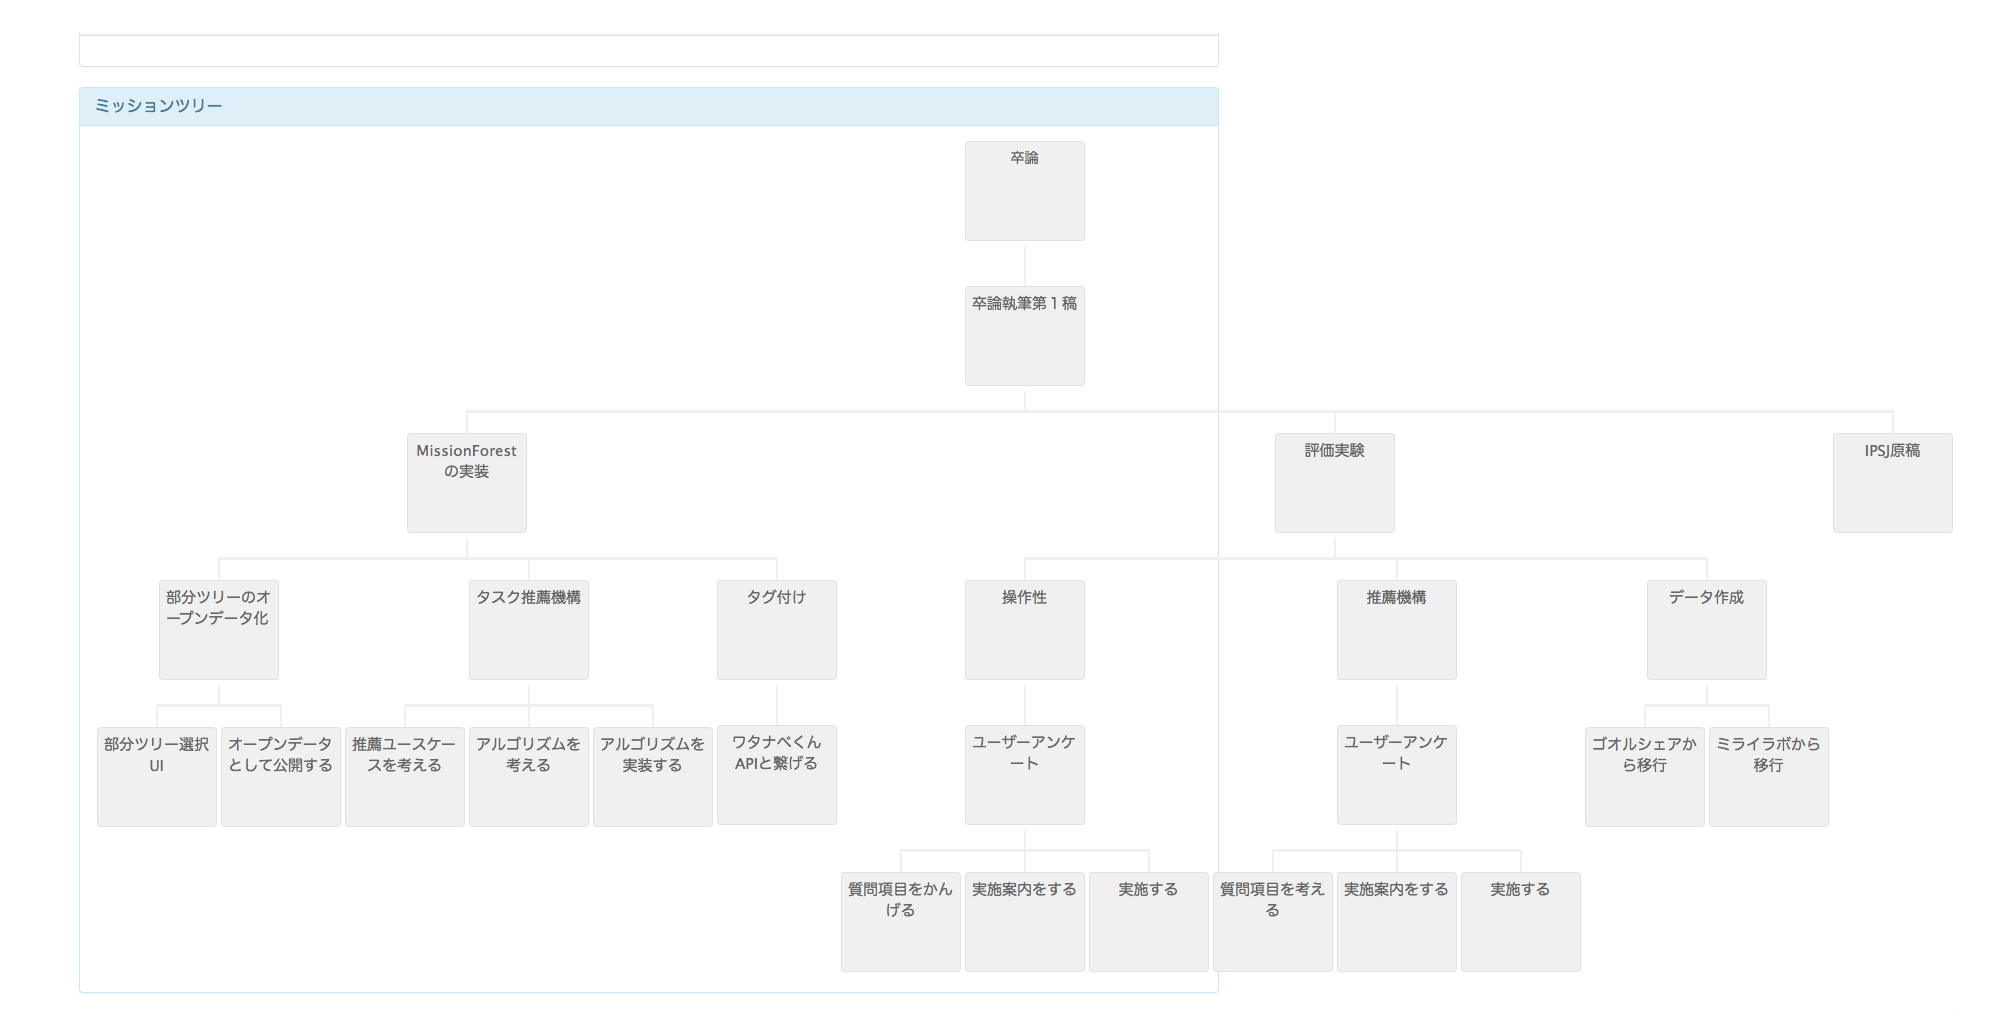
\includegraphics[width=0.9\linewidth]{assets/img/large_mission.png}
		\caption{ゴオルシェア実験結果}
		\label{img:large_mission}
	\end{center}
\end{figure}

\section{スキルタグ}
ユーザーはタスクに対して,そのタスクの完了に必要なスキルタグを登録することができる.

\section{ユーザースキルの重み付け}
ミッション内の完了したタスクについて,完了したユーザーがそのタスクに紐付いているスキルタグのスキルを有しているということになる.
このスキルタグを単純に出現回数順に推薦するのではなく,そのタスクの前後関係や,ミッション内での位置を考慮して重み付けを行う.
いかにそのアルゴリズムを述べる.

\subsection{重み付け関数}
